\documentclass[14pt]{extreport}
\usepackage{cmap}
\usepackage[utf8]{inputenc}
\usepackage[english,ukrainian]{babel}
\usepackage{graphicx}
\usepackage{geometry}
\usepackage{listings}
\usepackage{amsmath}
\usepackage{float}
\geometry{
	a4paper,
	left=20mm,
	right=20mm,
	top=20mm,
	bottom=20mm
}
\lstset{
	language=bash,
	tabsize=4,
	breaklines,
	keepspaces,
	showstringspaces=false,
}
\graphicspath{ {./pictures} }
\setlength{\parindent}{4em}

\newcommand\subject{Конструювання програмного забезпечення}
\newcommand\lecturer{доцент кафедри ПЗ\\Сердюк П.В.}
\newcommand\teacher{доцент кафедри ПЗ\\Сердюк П.В.}
\newcommand\mygroup{ПЗ-32}
\newcommand\lab{4}
\newcommand\theme{WPF}
\newcommand\purpose{Ознайомлення з засобами розробки WPF}

\begin{document}
\begin{normalsize}
	\begin{titlepage}
		\thispagestyle{empty}
		\begin{center}
			\textbf{МІНІСТЕРСТВО ОСВІТИ І НАУКИ УКРАЇНИ\\
				НАЦІОНАЛЬНИЙ УНІВЕРСИТЕТ "ЛЬВІВСЬКА ПОЛІТЕХНІКА"}
		\end{center}
		\begin{flushright}
			Інститут \textbf{КНІТ}\\
			Кафедра \textbf{ПЗ}
		\end{flushright}
		\vspace{200pt}
		\begin{center}
			\textbf{ЗВІТ}\\
			\vspace{10pt}
			До лабораторної роботи № \lab\\
			\textbf{На тему}: “\textit{\theme}”\\
			\textbf{З дисципліни}: “\subject”
		\end{center}
		\vspace{40pt}
		\begin{flushright}
			
			\textbf{Лектор}:\\
			\lecturer\\
			\vspace{10pt}
			\textbf{Виконав}:\\
			
			студент групи \mygroup\\
			Коваленко Д.М.\\
			\vspace{10pt}
			\textbf{Прийняв}:\\
			
			\teacher\\
			
			\vspace{28pt}
			«\rule{1cm}{0.15mm}» \rule{1.5cm}{0.15mm} 2023 р.\\
			$\sum$ = \rule{1cm}{0.15mm}……………\\
			
		\end{flushright}
		\vspace{\fill}
		\begin{center}
			\textbf{Львів — 2023}
		\end{center}
	\end{titlepage}
		
	\begin{description}
		\item[Тема.] \theme.
		\item[Мета.] \purpose.
	\end{description}

	\section*{Лабораторне завдання}
	Відповідно до варіанту проекту з баз даних 
	Потрібно реалізувати всі дії у відео на Youtube, але для свого варіанту проекту. Лабораторна може бути пов’язана з проектом бази даних або проектом з МПЗ/КПЗ. Повністю подібний код (який ідентичний тому що в Youtube не буде зарахований )
	
	\begin{enumerate}
		\item Реалізувати основні форми графічного інтерфейсу відповідно до проекту, наприклад: сплеш-скрін, головне меню, контекстне меню, меню закінчення рівня, і т.д.
		Реалізувати MVVM. Використовувати ICommand. Мінімально використовувати code behind.
		\item Основи розташування елементів. Використати компоненти StackPanel та Grid. Використати стилі. Не використовувати Margin для абсолютного вирівнювання (Margin > 30 вважається неприпустимим )
		\item Використання стилів - використати App.xml. 
		\item Використати компоненти DataGrid і зв’язування до даних. 
		\item Робота з ресурсами (як частини проекту, повинні бути компільовані у assembly, а не звертатися до них через шлях). Ресурси можуть бути звуками чи музикою. 
		\item Реалізувати конвертор
	\end{enumerate}
	
	
	\section*{Хід роботи}
	
	\begin{small}
		\begin{lstlisting}
		\end{lstlisting}
	\end{small}
	
	\begin{figure}[H]
		\centering
		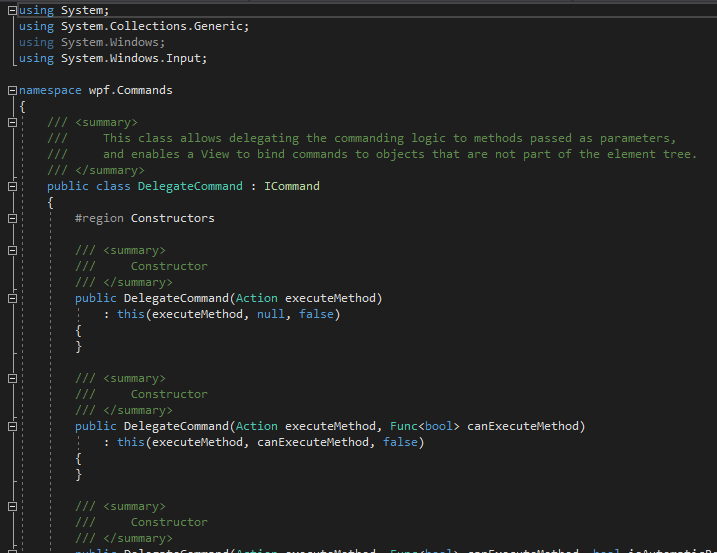
\includegraphics[scale=0.8]{1}
		\caption{Використання ICommand та DelegateCommand}
	\end{figure}
	
	
	\begin{figure}[H]
		\centering
		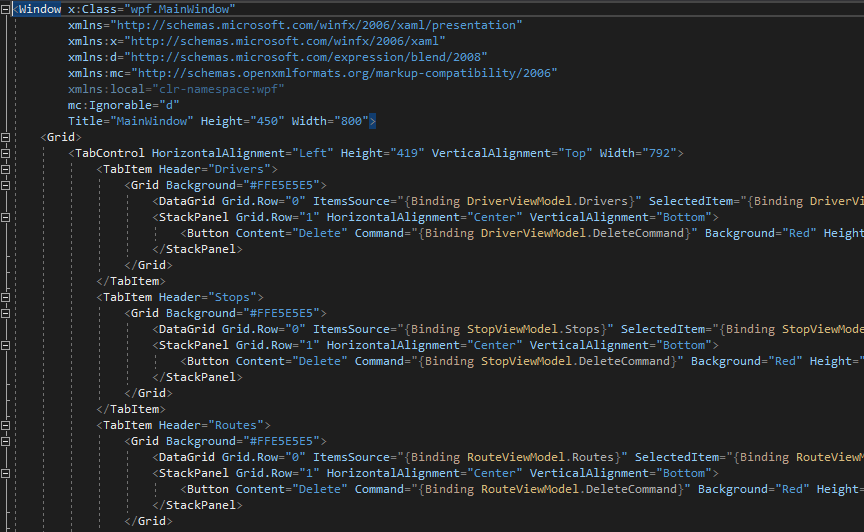
\includegraphics[scale=0.7]{2}
		\caption{Використання Стилів та datagrid, stackpanel, bindings}
	\end{figure}
	
	
	\begin{figure}[H]
		\centering
		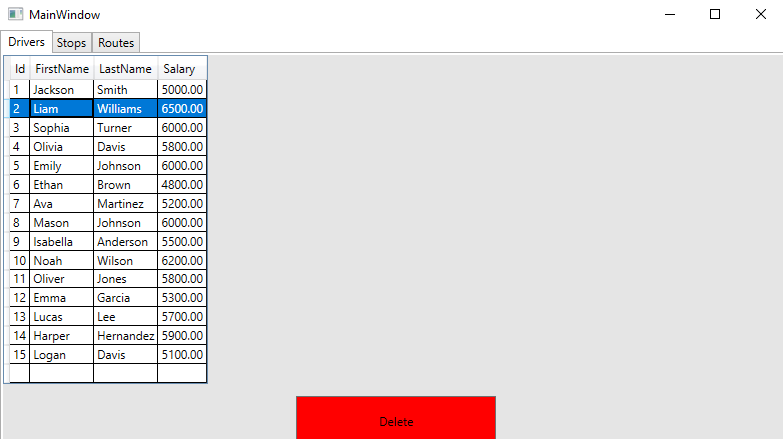
\includegraphics[scale=0.7]{3}
		\caption{Робота програми}
	\end{figure}
	
	\begin{figure}[H]
		\centering
		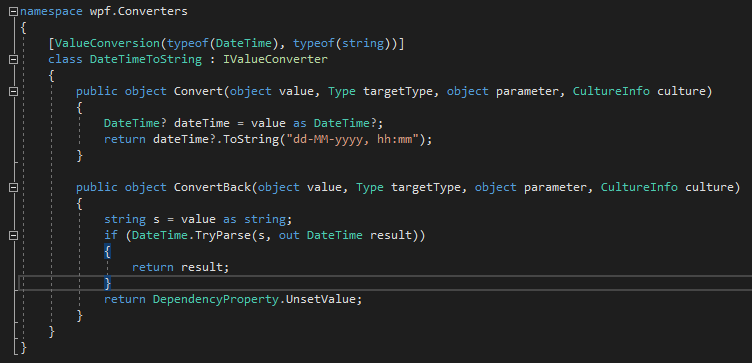
\includegraphics[scale=0.7]{4}
		\caption{Використання конвертора}
	\end{figure}
	\section*{Висновок}
	Виконуючи дану лабораторну роботу я дізнався структуру шаблону MVVM та реалізував програму відповідно до даного шаблону з використанням інтерфейсів ICommand, INotifyPropertyChanged.
	
	
	 
\end{normalsize}
\end{document}
